% Options for packages loaded elsewhere
\PassOptionsToPackage{unicode}{hyperref}
\PassOptionsToPackage{hyphens}{url}
%
\documentclass[
]{article}
\usepackage{amsmath,amssymb}
\usepackage{iftex}
\ifPDFTeX
  \usepackage[T1]{fontenc}
  \usepackage[utf8]{inputenc}
  \usepackage{textcomp} % provide euro and other symbols
\else % if luatex or xetex
  \usepackage{unicode-math} % this also loads fontspec
  \defaultfontfeatures{Scale=MatchLowercase}
  \defaultfontfeatures[\rmfamily]{Ligatures=TeX,Scale=1}
\fi
\usepackage{lmodern}
\ifPDFTeX\else
  % xetex/luatex font selection
\fi
% Use upquote if available, for straight quotes in verbatim environments
\IfFileExists{upquote.sty}{\usepackage{upquote}}{}
\IfFileExists{microtype.sty}{% use microtype if available
  \usepackage[]{microtype}
  \UseMicrotypeSet[protrusion]{basicmath} % disable protrusion for tt fonts
}{}
\makeatletter
\@ifundefined{KOMAClassName}{% if non-KOMA class
  \IfFileExists{parskip.sty}{%
    \usepackage{parskip}
  }{% else
    \setlength{\parindent}{0pt}
    \setlength{\parskip}{6pt plus 2pt minus 1pt}}
}{% if KOMA class
  \KOMAoptions{parskip=half}}
\makeatother
\usepackage{xcolor}
\usepackage[margin=1in]{geometry}
\usepackage{graphicx}
\makeatletter
\def\maxwidth{\ifdim\Gin@nat@width>\linewidth\linewidth\else\Gin@nat@width\fi}
\def\maxheight{\ifdim\Gin@nat@height>\textheight\textheight\else\Gin@nat@height\fi}
\makeatother
% Scale images if necessary, so that they will not overflow the page
% margins by default, and it is still possible to overwrite the defaults
% using explicit options in \includegraphics[width, height, ...]{}
\setkeys{Gin}{width=\maxwidth,height=\maxheight,keepaspectratio}
% Set default figure placement to htbp
\makeatletter
\def\fps@figure{htbp}
\makeatother
\setlength{\emergencystretch}{3em} % prevent overfull lines
\providecommand{\tightlist}{%
  \setlength{\itemsep}{0pt}\setlength{\parskip}{0pt}}
\setcounter{secnumdepth}{-\maxdimen} % remove section numbering
\usepackage{fontspec}
\setmainfont{Noto Sans CJK SC}
\usepackage{booktabs}
\usepackage{longtable}
\usepackage{array}
\usepackage{multirow}
\usepackage{wrapfig}
\usepackage{float}
\usepackage{colortbl}
\usepackage{pdflscape}
\usepackage{tabu}
\usepackage{threeparttable}
\usepackage{threeparttablex}
\usepackage[normalem]{ulem}
\usepackage{makecell}
\usepackage{xcolor}
\ifLuaTeX
  \usepackage{selnolig}  % disable illegal ligatures
\fi
\usepackage{bookmark}
\IfFileExists{xurl.sty}{\usepackage{xurl}}{} % add URL line breaks if available
\urlstyle{same}
\hypersetup{
  hidelinks,
  pdfcreator={LaTeX via pandoc}}

\author{}
\date{\vspace{-2.5em}}

\begin{document}

\section{前言}\label{ux524dux8a00}

在现代医学研究中,人体微生物组的作用受到了广泛关注,尤其是肠道菌群对宿主健康的影响。肠道菌群与宿主的新陈代谢、免疫功能以及某些疾病的发生发展,包括癌症,都有着密切的联系。甲状腺癌作为最常见的内分泌恶性肿瘤,其发病率近年来不断上升,这促使科研人员寻找新的生物标志物,以期改善诊断、预后评估和治疗策略。

本研究旨在探索肠道微生物群在甲状腺癌中的潜在标志物,我们通过分析与甲状腺癌相关的肠道菌群数据,尝试揭示肠道微生物与甲状腺癌之间的关联。我们从NCBI数据库获取了SRP151288号项目的原始fastq序列文件及其元数据,这为我们研究肠道微生物群提供了宝贵的数据资源。通过TOFU软件包中的Kraken2工具,我们对这些序列进行了精确的分类处理,生成了操作分类单元(OTU)表。与传统的菌群测序相比,Kraken2通过与数据库比对的方式进行分类,这可能在种(Species)水平上提供了更高的准确性,这一点与采用机器学习进行分类的dada2算法不同。

在构建了phyloseq对象之后,我们在属(Genus)和种(Species)两个分类级别上提取了微生物群落的关键特征。为了深入分析这些特征,我们采用了H2o平台的多种机器学习模型,包括广义线性模型、分布式随机森林、极端随机树和深度学习,以筛选出最优模型。我们还识别了在这些模型中共同显著的微生物特征,并通过非参数Wilcoxon检验对这些特征进行了验证,结果以箱线图形式展示,为我们提供了进一步统计学分析和解释的基础。
通过本研究,我们期望为甲状腺癌的诊断和治疗提供新的微生物学视角和潜在的生物标志物,同时也为肠道微生物组与癌症关系的研究领域贡献新的知识。

\section{方法学}\label{ux65b9ux6cd5ux5b66}

本研究首先从NCBI数据库检索并下载了SRP151288号项目的原始fastq序列文件及其相应的元数据(meta信息)。随后,利用TOFU软件包中的Kraken2工具对这些fastq序列进行了分类处理,生成了操作分类单元(OTU)表。此OTU表接着被导入到phyloseq包中,以构建phyloseq对象,便于后续分析。在phyloseq环境下,我们分别在属(Genus)和种(Species)两个分类级别上,提取了微生物群落的关键特征。为了对这些关键特征进行深入分析,我们采用了H2o平台,通过多种机器学习模型,包括广义线性模型(Generalized
Linear Model)、分布式随机森林(Distributed Random
Forest)、极端随机树(eXtremely Randomized
Trees)和深度学习(DeepLearning),进行了模型训练,旨在筛选出最优模型。此外,我们还识别了在这些模型中共同显著的微生物特征,并对这些一致性特征进行了非参数Wilcoxon检验,结果以箱线图(boxplot)形式展示,以便于进一步的统计学分析和解释。

\section{流程图}\label{ux6d41ux7a0bux56fe}

\begin{figure}
\centering
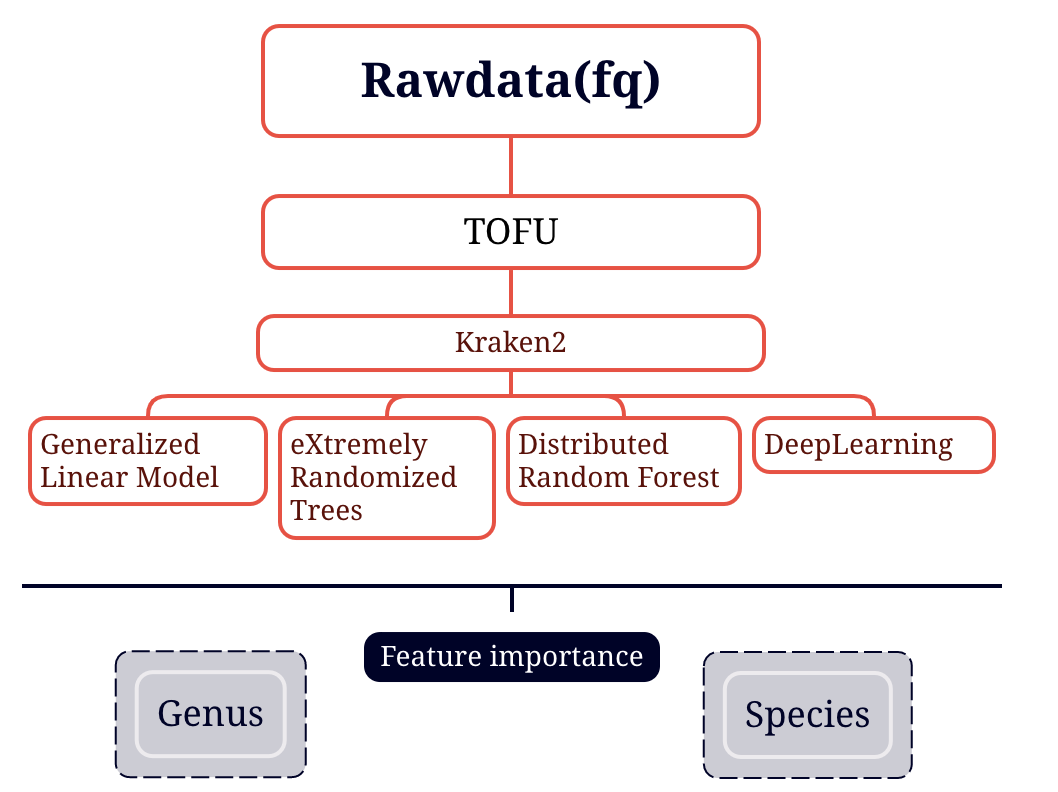
\includegraphics[width=1\textwidth,height=1\textheight]{../input/流程图/Litao_流程图.png}
\caption{Figure1: 图片标题}
\end{figure}

\section{结果部分}\label{ux7ed3ux679cux90e8ux5206}

\subsection{基于属水平的机器学习特征选择}\label{ux57faux4e8eux5c5eux6c34ux5e73ux7684ux673aux5668ux5b66ux4e60ux7279ux5f81ux9009ux62e9}

\subsubsection{基于多种模型特征的模型评价}\label{ux57faux4e8eux591aux79cdux6a21ux578bux7279ux5f81ux7684ux6a21ux578bux8bc4ux4ef7}

\begin{figure}
\centering
\includegraphics[width=1\textwidth,height=1\textheight]{../../Kraken/output/H20/SRP151288_HC_vs_TC.Genus/df_scores_model_barplot.png-1.png}
\caption{Table1:
AutoML生成的机器学习模型性能指标。模型基于AUC和平均每类错误率进行评估,排名首位的模型AUC约为0.996。}
\end{figure}

\subsubsection{基于多种模型特征的重要性热图}\label{ux57faux4e8eux591aux79cdux6a21ux578bux7279ux5f81ux7684ux91cdux8981ux6027ux70edux56fe}

\begin{figure}
\centering
\includegraphics[width=1\textwidth,height=1\textheight]{../../Kraken/output/H20/SRP151288_HC_vs_TC.Genus/H20_feature_importance_heatmap_plot.png-1.png}
\caption{Figure2: Heatmap of Feature Importance Based on Multiple Models
This heatmap displays the importance ranking of various features in
different machine learning models for predicting thyroid cancer. The
darker the color, the higher the importance of the feature in the
model.}
\end{figure}

\subsubsection{基于多种模型共有特征的boxplot}\label{ux57faux4e8eux591aux79cdux6a21ux578bux5171ux6709ux7279ux5f81ux7684boxplot}

\begin{figure}
\centering
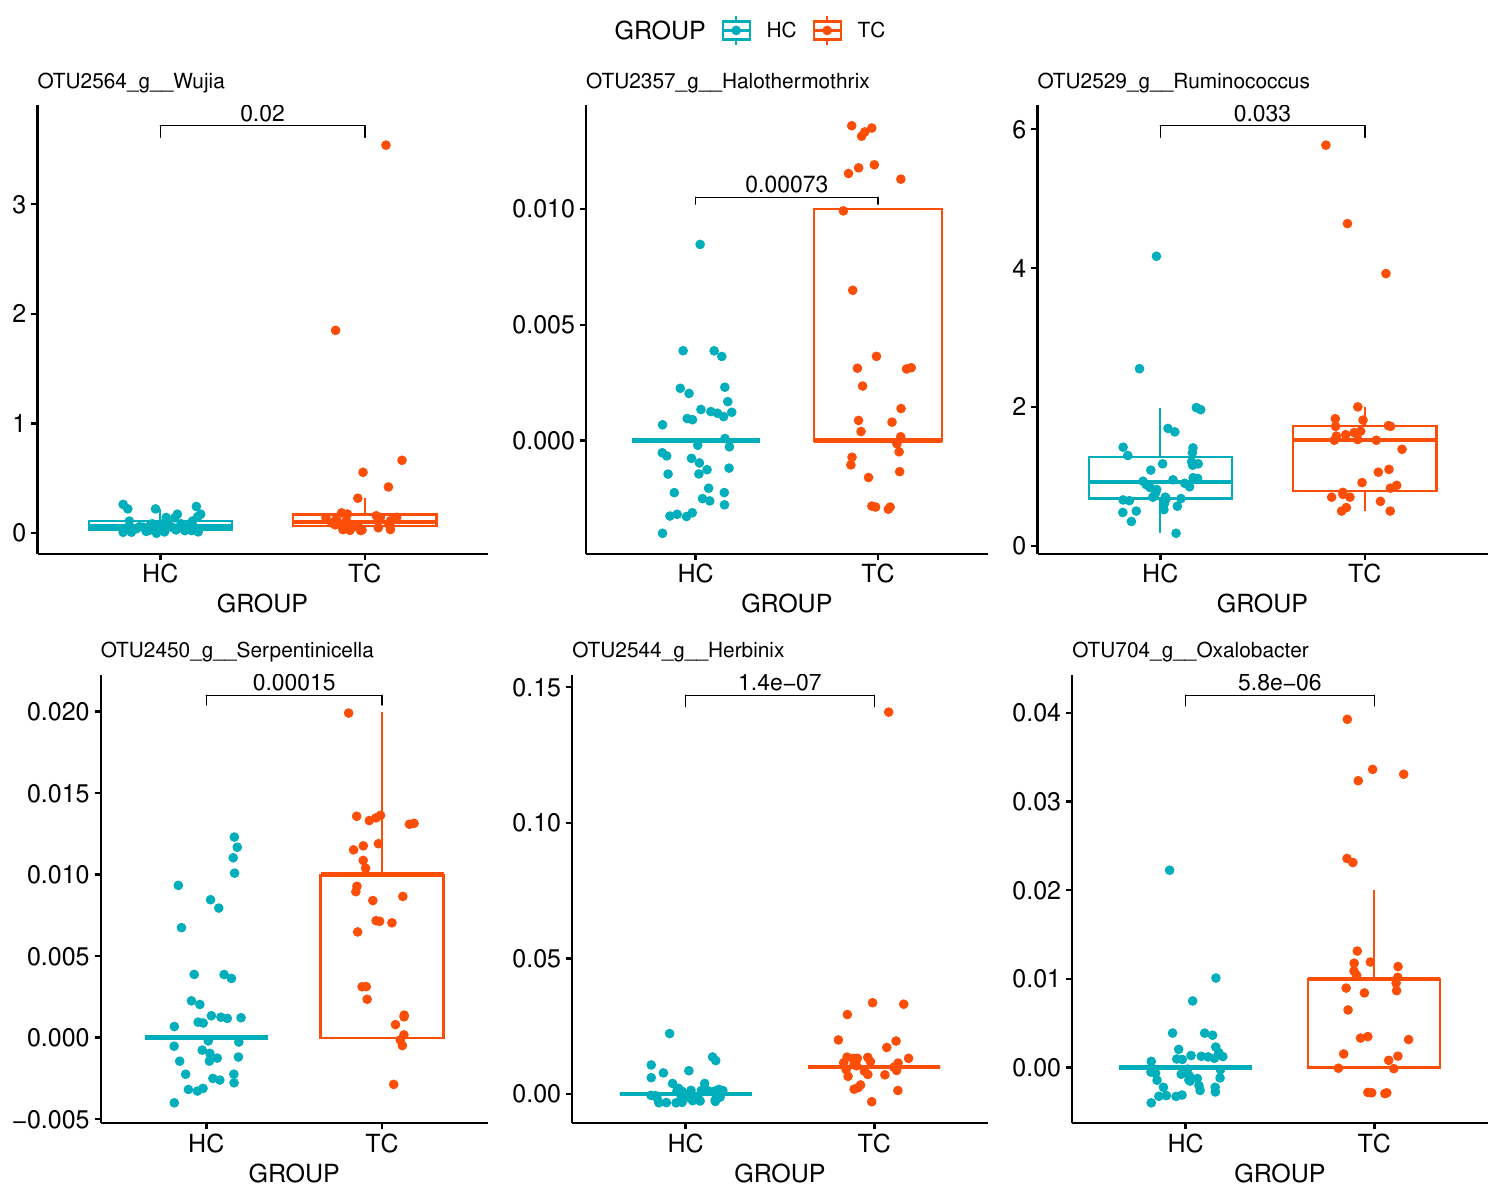
\includegraphics[width=1\textwidth,height=1\textheight]{../../Kraken/output/H20/SRP151288_HC_vs_TC.Genus/Genus_boxplot.png-1.png}
\caption{Figure3: Boxplot of Shared Features Based on Multiple Models
The boxplot compares the expression differences of important shared
features between the healthy control group and the thyroid cancer
patient group across multiple models. The plot reveals significant
differences in some key features between the two groups, providing a
basis for subsequent statistical analysis.}
\end{figure}

\subsubsection{基于多种模型特征的ROC曲线}\label{ux57faux4e8eux591aux79cdux6a21ux578bux7279ux5f81ux7684rocux66f2ux7ebf}

\begin{figure}
\centering
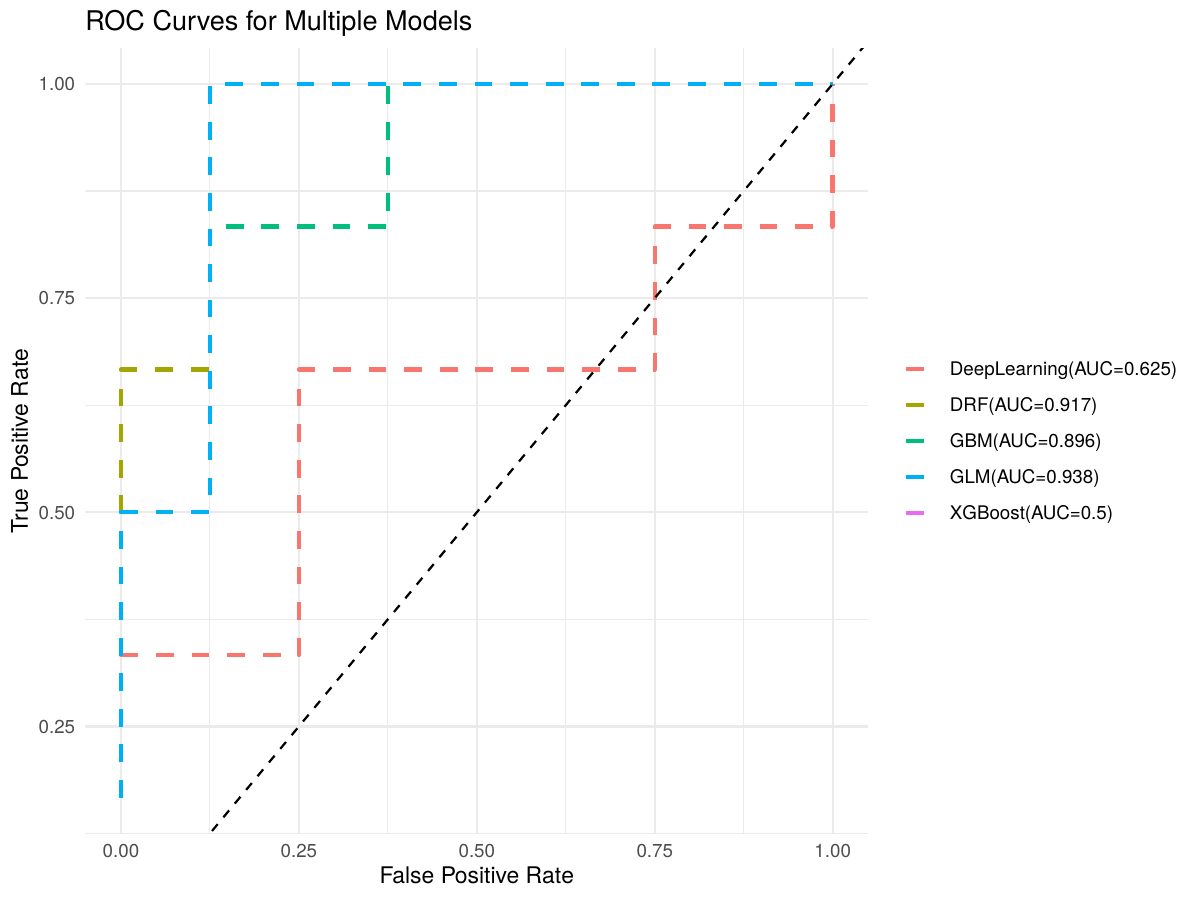
\includegraphics[width=1\textwidth,height=1\textheight]{../../Kraken/output/H20/SRP151288_HC_vs_TC.Genus/H20_ROC_models_Genus.png-1.png}
\caption{Figure4: ROC Curve Based on the Optimal Model The Receiver
Operating Characteristic (ROC) curve reflects the performance of the
chosen optimal model in the task of predicting thyroid cancer. An Area
Under the Curve (AUC) value close to 1 indicates that the model can
effectively distinguish between the healthy population and patients.}
\end{figure}

\subsubsection{基于最优模型的热图重要性排序}\label{ux57faux4e8eux6700ux4f18ux6a21ux578bux7684ux70edux56feux91cdux8981ux6027ux6392ux5e8f}

\begin{figure}
\centering
\includegraphics[width=1\textwidth,height=1\textheight]{../../Kraken/output/H20/SRP151288_HC_vs_TC.Genus/H20_feature_importance_heatmap_plot.png-1.png}
\caption{Figure5: Heatmap of Feature Importance Based on the Optimal
Model This heatmap shows the importance ranking of various features in
the optimal prediction model. The y-axis shows the names of the
variables/features. The x-axis displays the variable importance scores
for each variable, with the score values ranging from 0.00 to 1.00. It
visually indicates which features have the greatest impact on the
predictive performance of the model.}
\end{figure}

\subsection{基于种水平的机器学习特征选择}\label{ux57faux4e8eux79cdux6c34ux5e73ux7684ux673aux5668ux5b66ux4e60ux7279ux5f81ux9009ux62e9}

\subsubsection{基于多种模型特征的模型评价}\label{ux57faux4e8eux591aux79cdux6a21ux578bux7279ux5f81ux7684ux6a21ux578bux8bc4ux4ef7-1}

\begin{figure}
\centering
\includegraphics[width=1\textwidth,height=1\textheight]{../../Kraken/output/H20/SRP151288_HC_vs_TC.Species/df_scores_model_barplot.png-1.png}
\caption{Table2:
AutoML生成的机器学习模型性能指标。模型基于AUC和平均每类错误率进行评估,排名首位的模型AUC约为0.996。}
\end{figure}

\subsubsection{基于多种模型特征的重要性热图}\label{ux57faux4e8eux591aux79cdux6a21ux578bux7279ux5f81ux7684ux91cdux8981ux6027ux70edux56fe-1}

\begin{figure}
\centering
\includegraphics[width=1\textwidth,height=1\textheight]{../../Kraken/output/H20/SRP151288_HC_vs_TC.Species/H20_feature_importance_heatmap_plot.png-1.png}
\caption{Figure6: Heatmap of Feature Selection Importance Based on
Species Level Figure 6 displays the evaluation of feature importance by
different models at the species level. In the heatmap, the darker the
color, the higher the importance of the feature in the model. This helps
us understand which features are important at the species level}
\end{figure}

\subsubsection{基于多种模型共有特征的boxplot}\label{ux57faux4e8eux591aux79cdux6a21ux578bux5171ux6709ux7279ux5f81ux7684boxplot-1}

\begin{figure}
\centering
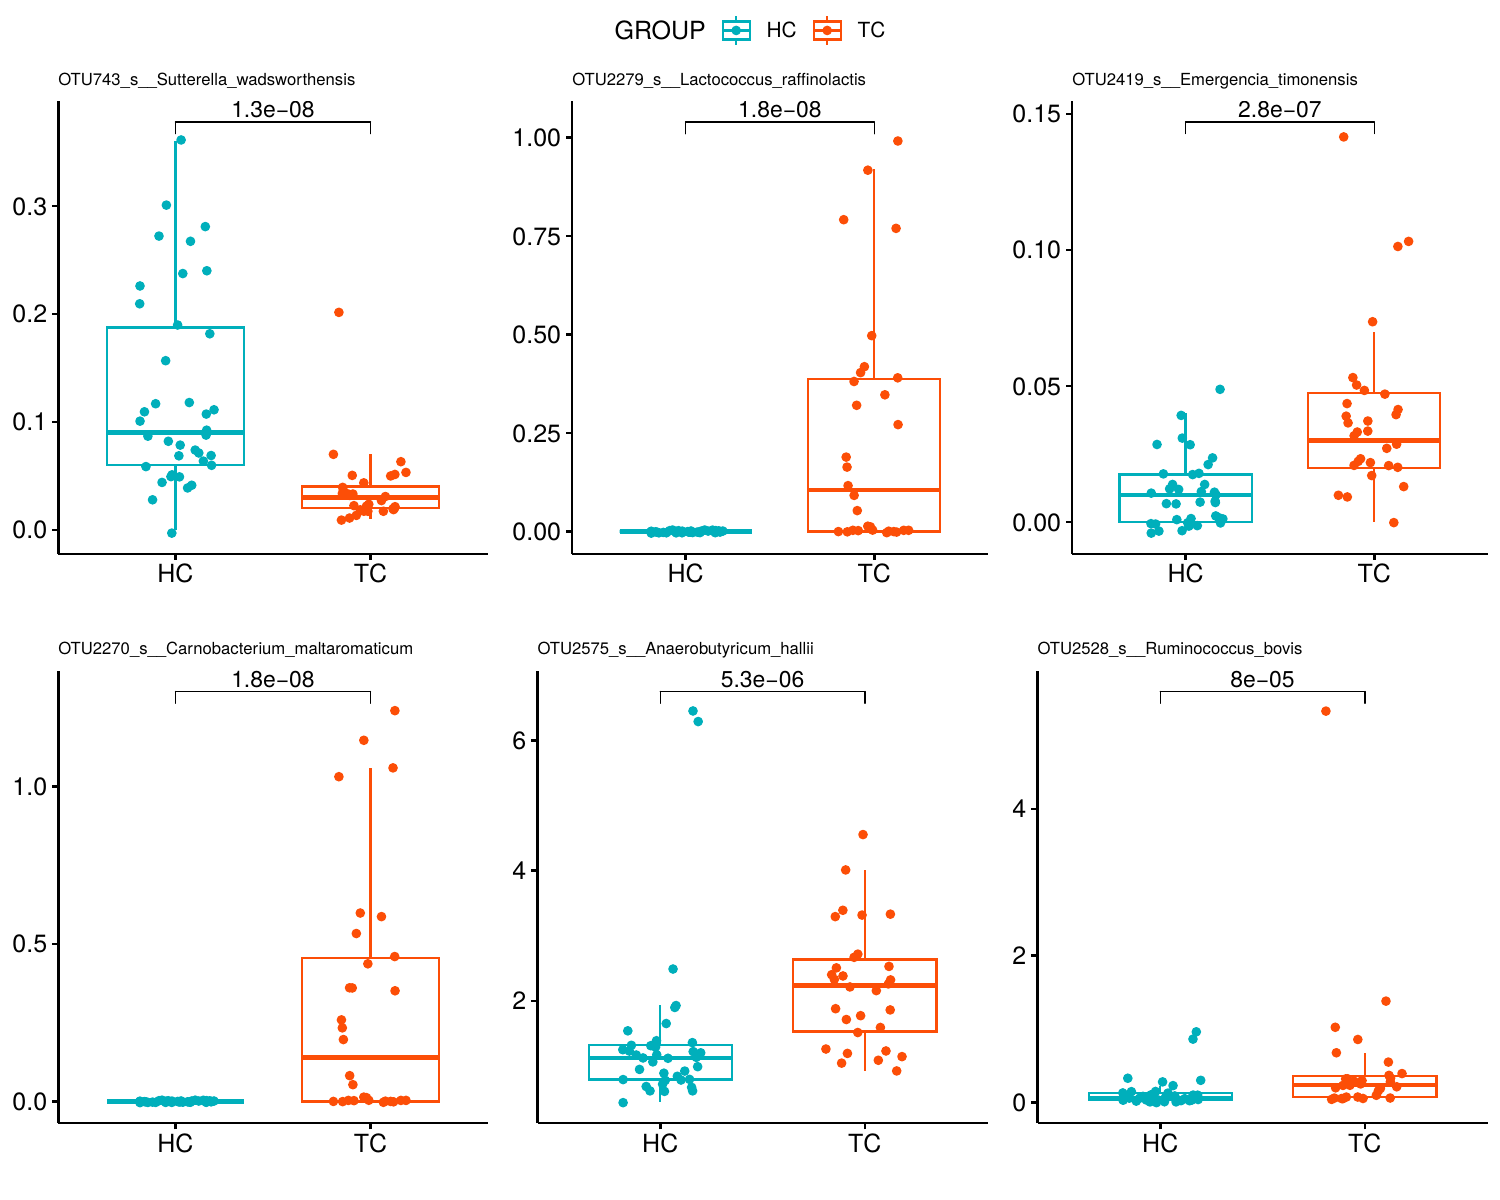
\includegraphics[width=1\textwidth,height=1\textheight]{../../Kraken/output/H20/SRP151288_HC_vs_TC.Species/Species_boxplot.png-1.png}
\caption{Figure7: Boxplot of Shared Features Based on Multiple Models at
Species Level This boxplot shows the expression differences of important
shared features between the healthy control group and the thyroid cancer
patient group across multiple models at the species level.}
\end{figure}

\subsubsection{基于多种模型特征的ROC曲线}\label{ux57faux4e8eux591aux79cdux6a21ux578bux7279ux5f81ux7684rocux66f2ux7ebf-1}

\begin{figure}
\centering
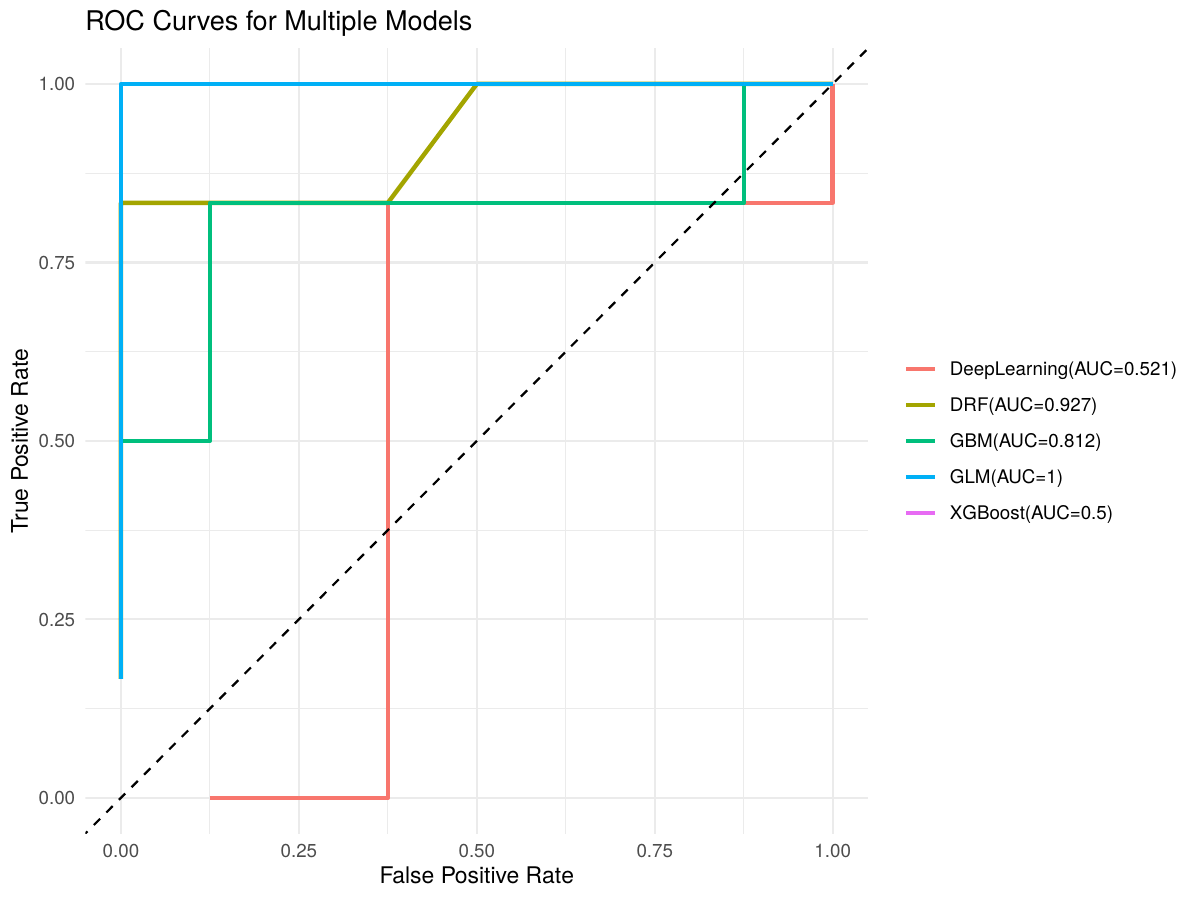
\includegraphics[width=1\textwidth,height=1\textheight]{../../Kraken/output/H20/SRP151288_HC_vs_TC.Species/H20_ROC_models_Species.png-1.png}
\caption{Figure8: ROC Curve Based on the Optimal Model at Species Level
The Receiver Operating Characteristic (ROC) curve reflects the
performance of the chosen optimal model at the species level in the task
of predicting thyroid cancer. An Area Under the Curve (AUC) value close
to 1 indicates that the model can effectively distinguish between the
healthy population and patients at the species level.}
\end{figure}

\subsubsection{基于最优模型的热图重要性排序}\label{ux57faux4e8eux6700ux4f18ux6a21ux578bux7684ux70edux56feux91cdux8981ux6027ux6392ux5e8f-1}

\begin{figure}
\centering
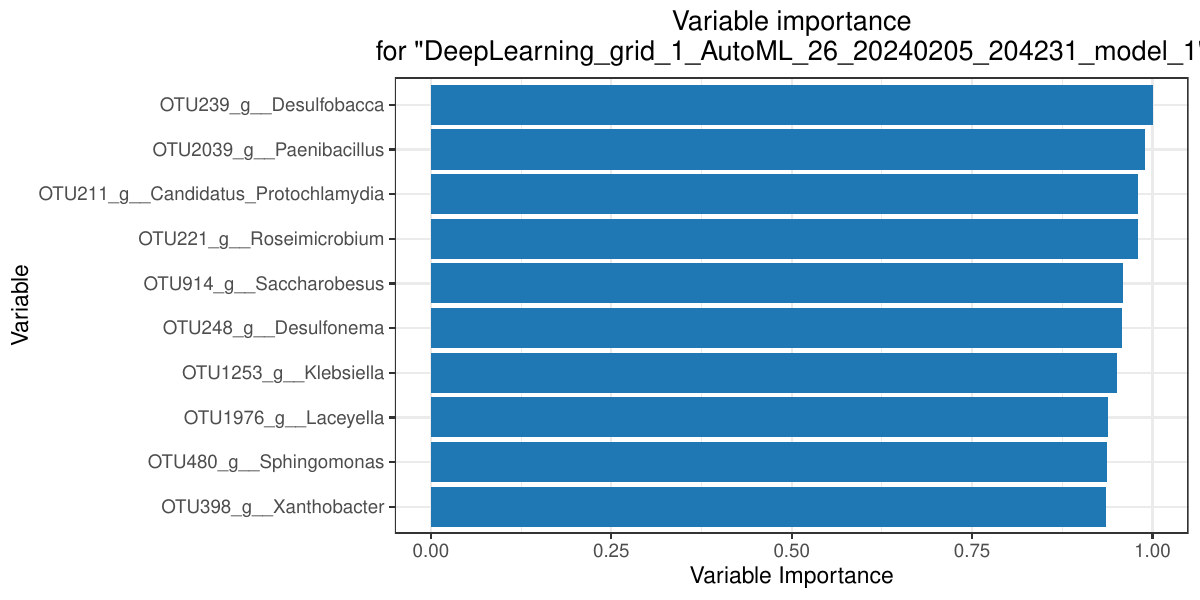
\includegraphics[width=1\textwidth,height=1\textheight]{../../Kraken/output/H20/SRP151288_HC_vs_TC.Species/H20_featur_importance_plot.png-1.png}
\caption{Figure9: Heatmap of Feature Importance Based on the Optimal
Model at Species Level This heatmap shows the importance ranking of
various features in the optimal prediction model at the species level.
The y-axis shows the names of the variables/features. The x-axis
displays the variable importance scores for each variable, with the
score values ranging from 0.00 to 1.00. It visually indicates which
features have the greatest impact on the predictive performance of the
model at this level}
\end{figure}

\end{document}
